% Unofficial University of Cambridge Poster Template
% https://github.com/andiac/gemini-cam
% a fork of https://github.com/anishathalye/gemini
% also refer to https://github.com/k4rtik/uchicago-poster

\documentclass[final]{beamer}

% ====================
% Packages
% ====================

\usepackage[T1]{fontenc}
\usepackage{lmodern}
\usepackage[orientation=portrait,size=a1,scale=1.0]{beamerposter}
\usetheme{gemini}
\usecolortheme{nott}
\usepackage{graphicx}
\usepackage{booktabs}
\usepackage{tikz}

\usepackage{pgfplots}
\pgfplotsset{compat=1.14}
\usepackage{anyfontsize}

% ====================
% Lengths
% ====================

% If you have N columns, choose \sepwidth and \colwidth such that
% (N+1)*\sepwidth + N*\colwidth = \paperwidth
\newlength{\sepwidth}
\newlength{\colwidth}
\setlength{\sepwidth}{0\paperwidth}
\setlength{\colwidth}{0.30\paperwidth}

\newcommand{\separatorcolumn}{\begin{column}{\sepwidth}\end{column}}

% ====================
% Title
% ====================

\title{Using Adversarial Attacks as Data Augmentation Methods for Deep Learning}

\author{Student: Zhongbo Yan, Steve \and Supervisor: Xu Yang \and Assessor: Liam Lei}

\institute[shortinst]{Bachelor of Science in Computing (2022-2023) \samelineand Macao Polytechnic University \and Email: P1908326@mpu.edu.mo | me@aspires.cc}

% ====================
% Footer (optional)
% ====================

\footercontent{
  \href{https://mpu.edu.mo}{Macao Polytechnic University} \hfill
  https://github.com/Ex10si0n/research \hfill
  \href{mailto:me@aspires.cc}{me@aspires.cc}}
% (can be left out to remove footer)


% ====================
% Logo (optional)
% ====================

% use this to include logos on the left and/or right side of the header:
% \logoright{\includegraphics[height=7cm]{logos/NCG-LOGO-INV.pdf}}
\logoleft{
\includegraphics[height=9cm]{mpu.png}}

% ====================
% Body
% ====================

\begin{document}

% Refer to https://github.com/k4rtik/uchicago-poster
% logo: https://www.cam.ac.uk/brand-resources/about-the-logo/logo-downloads
% \addtobeamertemplate{headline}{}
% {
%     \begin{tikzpicture}[remember picture,overlay]
%       \node [anchor=north west, inner sep=3cm] at ([xshift=-2.5cm,yshift=1.75cm]current page.north west)
%       {\includegraphics[height=7cm]{logos/unott-logo.eps}}; 
%     \end{tikzpicture}
% }

\begin{frame}[t]
\begin{columns}[t]
\separatorcolumn

\begin{column}{\colwidth}

  \begin{block}{Abstract}

    Adversarial attacks can be used to deceive deep learning models, producing incorrect predictions. By generating imperceptible perturbations to original images, these attacks can serve as an effective data augmentation method for enlarging training datasets by giving the attacked image a true label, hence improving the performance of image classification models. In this project, an adversarial training method was evaluated using the MRNet dataset for knee MRI images. Using FGSM attack, extra perturbed images were generated for retraining a well-trained CNN model. Results showed improved \textbf{accuracy}, \textbf{AUC}, \textbf{sensitivity}, and \textbf{specificity} compared to the baseline model provided by the Stanford Machine Learning Group.

    
  \end{block}
  \begin{block}{Introduction}

    Magnetic resonance imaging (MRI) of the knee is the standard care imaging modality to evaluate knee disorders. More musculoskeletal MR examinations are performed on the knee than on any other body region. 
    
    \textbf{The MRNet dataset}, provided by the Stanford ML Group, contains knee MRI examinations used to determine abnormal categories. The dataset has been split into the training (1130 exams) dataset and the validation (120 exams) dataset. 
    
    In addition, in each exam, there are MR images in three planes, namely \textbf{axial}, \textbf{coronal}, and \textbf{sagittal}, for classifying three types of abnormality (\textbf{abnormal}: 80.6\%, \textbf{ACL tears}: 23.3\%, and \textbf{meniscal tears}: 37.1\%) obtained through manual extraction from clinical reports.
    
    \begin{table}
      \centering
      \begin{tabular}{l r r r}
        \toprule
        \textbf{Planes/Tasks} & \textbf{Abnormal} & \textbf{ACL tears} & \textbf{Meniscal} \\
        \midrule
        \textbf{Axial} & $\text{Model}_{A1}$ & $\text{Model}_{A2}$ & $\text{Model}_{A3}$ \\
        \textbf{Coronal} & $\text{Model}_{C1}$ & $\text{Model}_{C2}$ & $\text{Model}_{C3}$ \\
        \textbf{Sagittal} & $\text{Model}_{S1}$ & $\text{Model}_{S2}$ & $\text{Model}_{S3}$ \\
        \bottomrule
      \end{tabular}
      \caption{MRNet Binary Classification Models}
    \end{table}

    \begin{figure}[!htp]
    \centering
    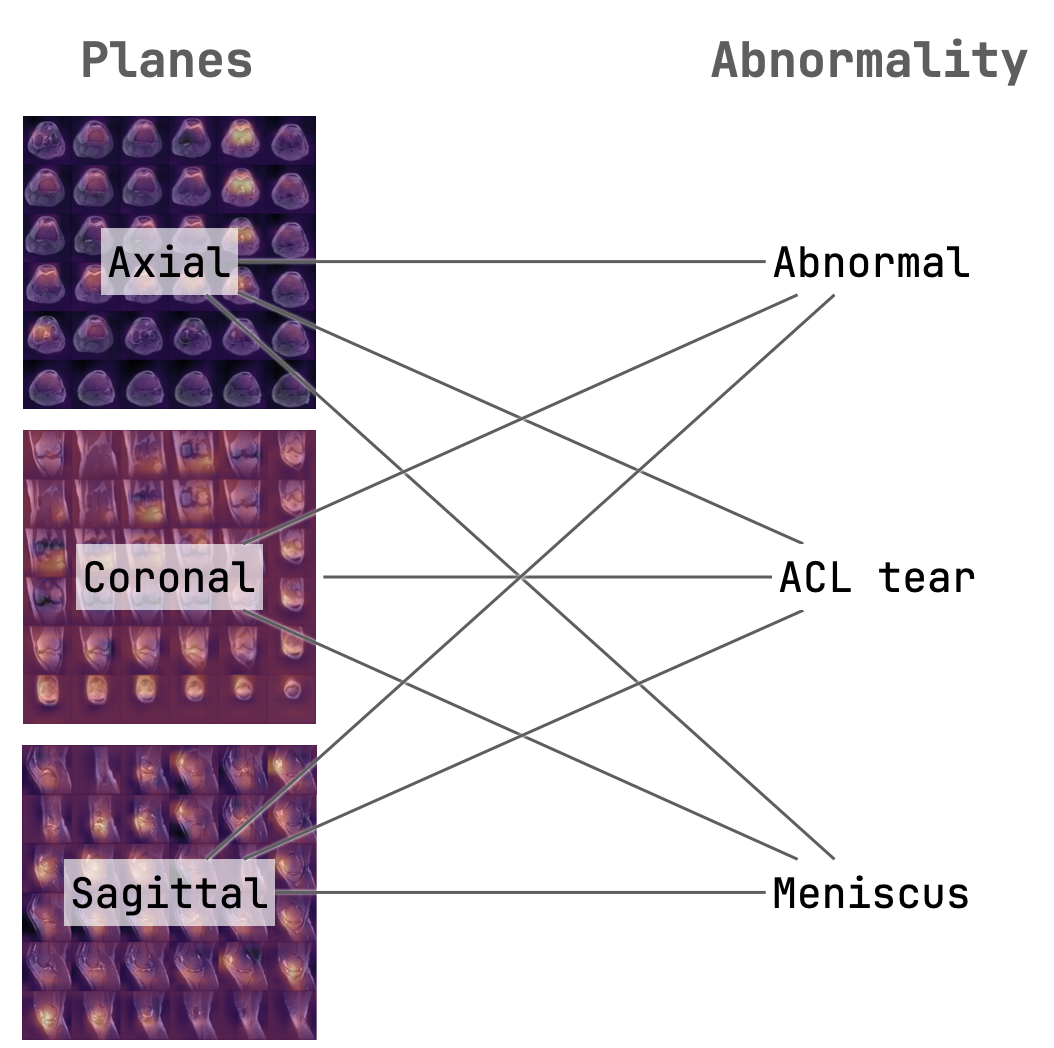
\includegraphics[width=0.8\textwidth]{dataset_visual.png}
    \caption{\label{fig:dataset}MRNet Dataset}
    \end{figure}

    \textbf{Baseline Model} of this project is the best model [mrnet-baseline (single model) Stanford University, AUC: 0.917] released on the ranking board of MRNet. The code of the baseline model can be found on GitHub: \href{https://github.com/matteo-dunnhofer/mrnet-baseline}{\verb|matteo-dunnhofer/mrnet-baseline|}

    \begin{figure}[!htp]
    \centering
    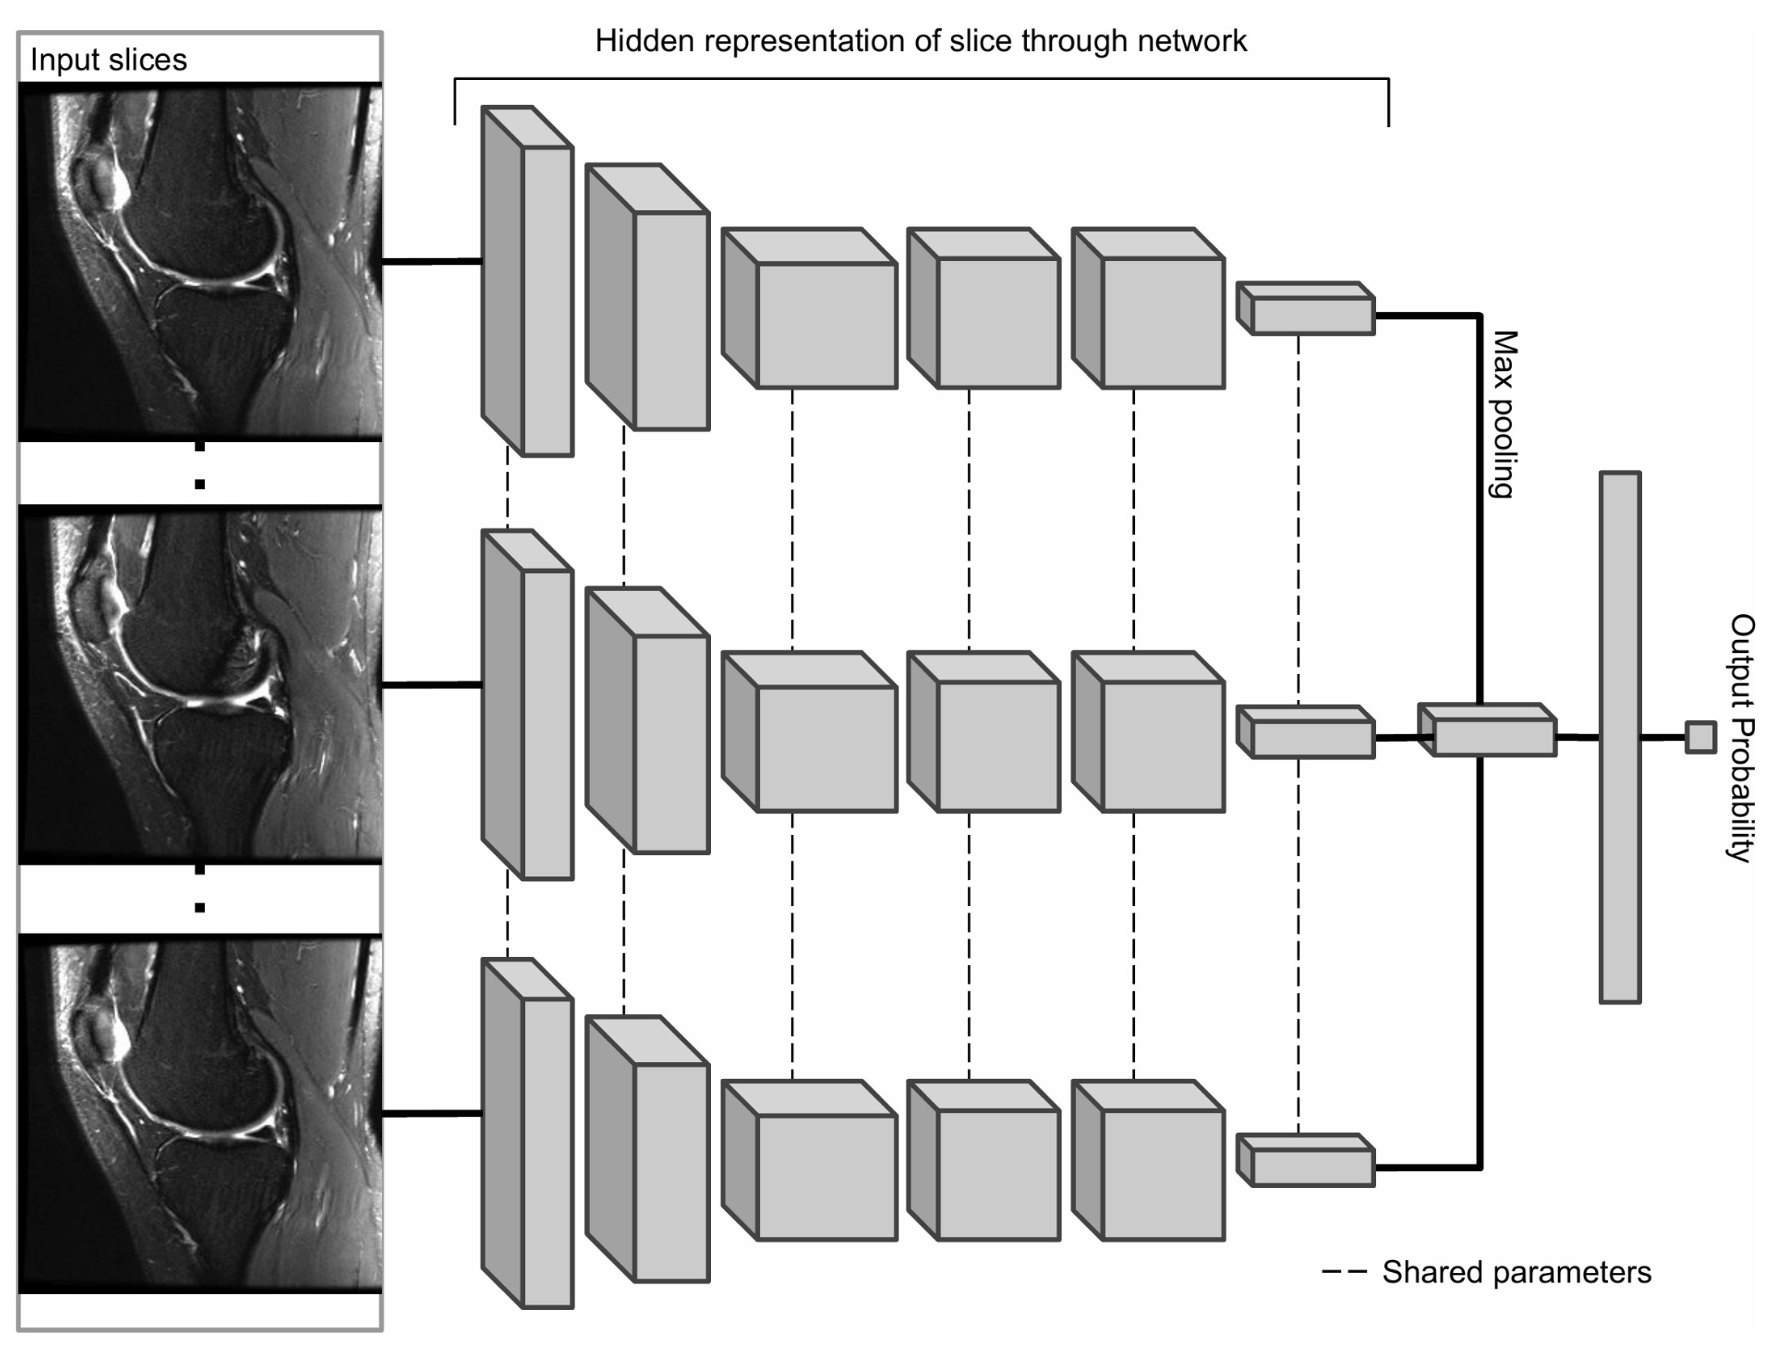
\includegraphics[width=1\textwidth]{mrnet.png}
    \caption{\label{fig:dataset}Baseline Network Visualization}
    \end{figure}

    This project's experiment involves training a baseline model using its conventional data augmentation techniques. Afterwards, the models are retrained with a particular portion of data, known as the retrain percentage, which is perturbed with a specific Fast Gradient Sign Method (FGSM) attack rate denoted as epsilon (\epsilon). The objective of this experiment is to assess the effect of re-training using adversarial examples on the MRNet model's performance.

    
  \end{block}

 

\end{column}

\separatorcolumn

\begin{column}{\colwidth}

  \begin{block}{Problem}

    In 2019, Tasnim et al. proposed InvFGSM technique for medical image segmentation. In 2020, Xie et al. introduced AdvProp to improve recognition accuracy using separate batches for original data and adversarial examples generated by PGD attacks. Gong et al. introduced MaxUp, which updated neural network parameters using augmented data with perturbations by maximum loss of each batch. 

    In the literature, the current published works only evaluate the performance improvement of accuracy and AUC. the impact on other metrics such as sensitivity, and specificity have not been studied, to the best knowledge of the author. Additionally, there has been no previous research conducted on medical Magnetic Resonance Imaging (MRI) classification tasks using adversarial data augmentation.
    

  \end{block}

  \begin{block}{Algorithm \& Implementation}

    \textbf{The Fast Gradient Sign Method (FGSM)}, introduced by Ian Goodfellow et al. is one of the most popular adversarial attack methods, which aims to generate malicious examples by perturbing the input data to maximum gradient of loss. The carefully crafted perturbation is designed to be small enough to be visually imperceptible to humans, while still being large enough to cause the model to misclassify the input.

    \begin{equation}
    X_{adv} = X + \epsilon \times sign(\nabla_X J(\theta, X, y))
    \end{equation}
    (1) Equation of generating adversarial examples using FGSM
    \begin{itemize}
        \item \makebox[3.2cm]{\textbf{$X_{adv}$}\hfill} adversarial example generated using the FGSM
        \item \makebox[3.2cm]{\textbf{$X$}\hfill} original input example
        \item \makebox[3.2cm]{\textbf{\epsilon}\hfill} the magnitude of the perturbation
        \item \makebox[3.2cm]{\textbf{$sign()$}\hfill} function that returns the +/- sign of its argument
        \item \makebox[3.2cm]{\textbf{$\nabla_x J(θ, X, y)$}\hfill} gradient of the model's loss function $J$
        \item \makebox[3.2cm]{\textbf{$\theta$}\hfill} model parameters
        \item \makebox[3.2cm]{\textbf{$X, y$}\hfill} input data, true labels
    \end{itemize}
    
    \begin{figure}[!htp]
    \centering
    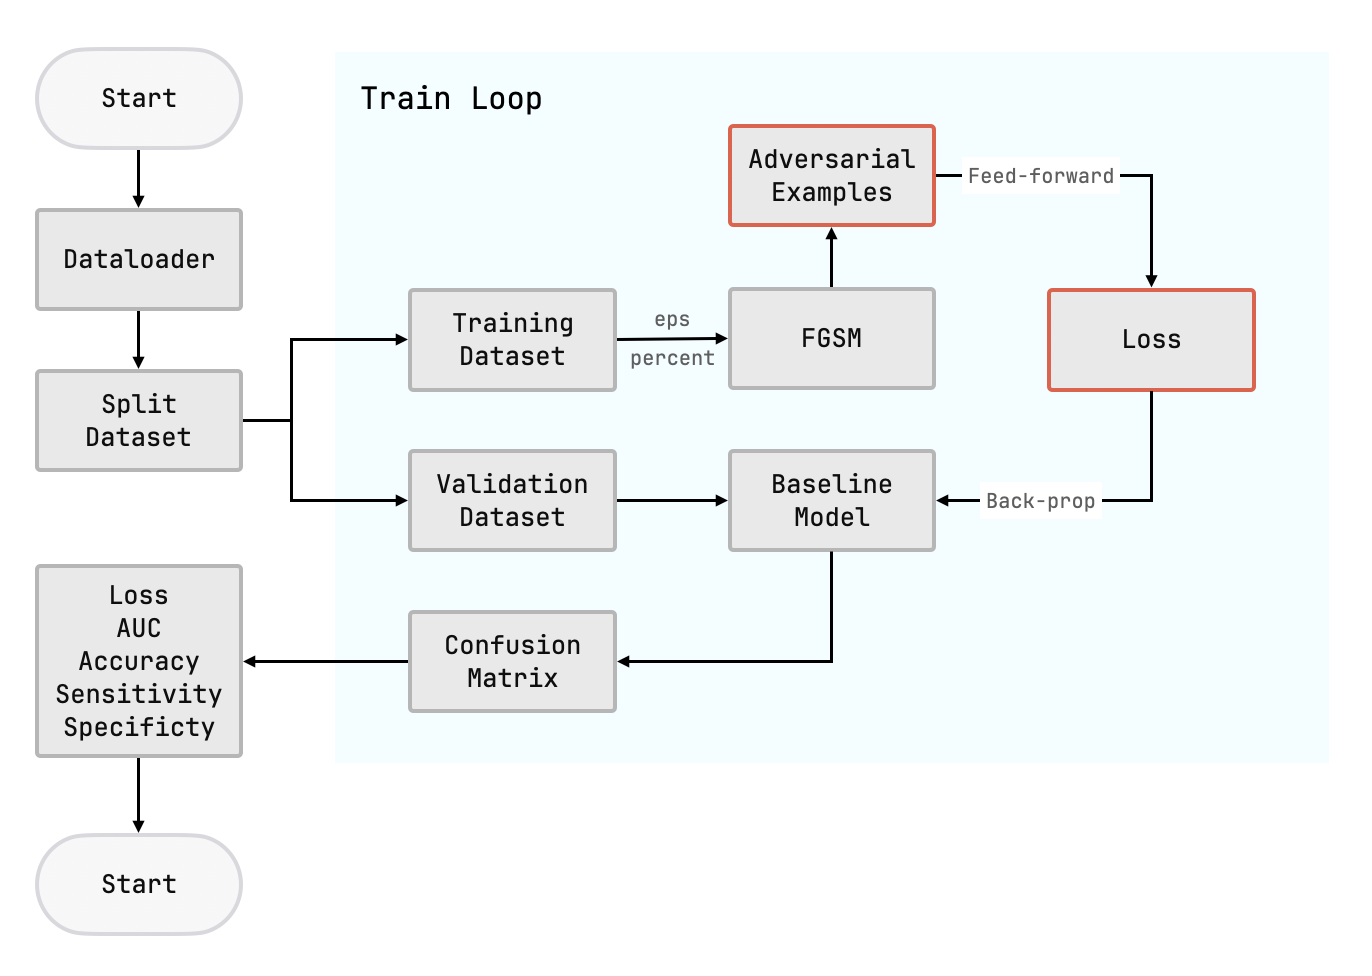
\includegraphics[width=0.95\textwidth]{diagram.png}
    \caption{\label{fig:adv}Experiment Flow Chart}
    \end{figure}

    \textbf{Adversarial training} is a technique that aims to make models more robust to these attacks by training them on adversarial examples (perturbed input). The diagram [Figure 3] illustrates this procedure. 

    The adversarial training process is performed for each epoch, following these steps, where $\mu$ is the learning rate, $\theta$ is the model parameter, and $(X_i, y_i)$ is a batch of training data determined by the hyperparameter for the retrain percentage.
    \begin{align}
        \delta_{i}^{FGSM} &:= \epsilon \times sign(\nabla_{X_i}J(X_i, y_i, \theta)) \\
        X_{i}^{adv} &:= X_i + \delta_{m}^{FGSM} \\
        \theta &:= \theta - \mu \nabla_\theta J(X_i^{adv}, y_i, \theta)
    \end{align}
    
    (2) Generating adversarial perturbations $\delta_{i}^{FGSM}$ for training data $X_i$
    
    (3) Generating adversarial examples $X_i^{adv}$
    
    (4) Updating (Gradient Descent) Model's parameters $\theta$
    
    % \begin{figure}[!htp]
    % \centering
    % 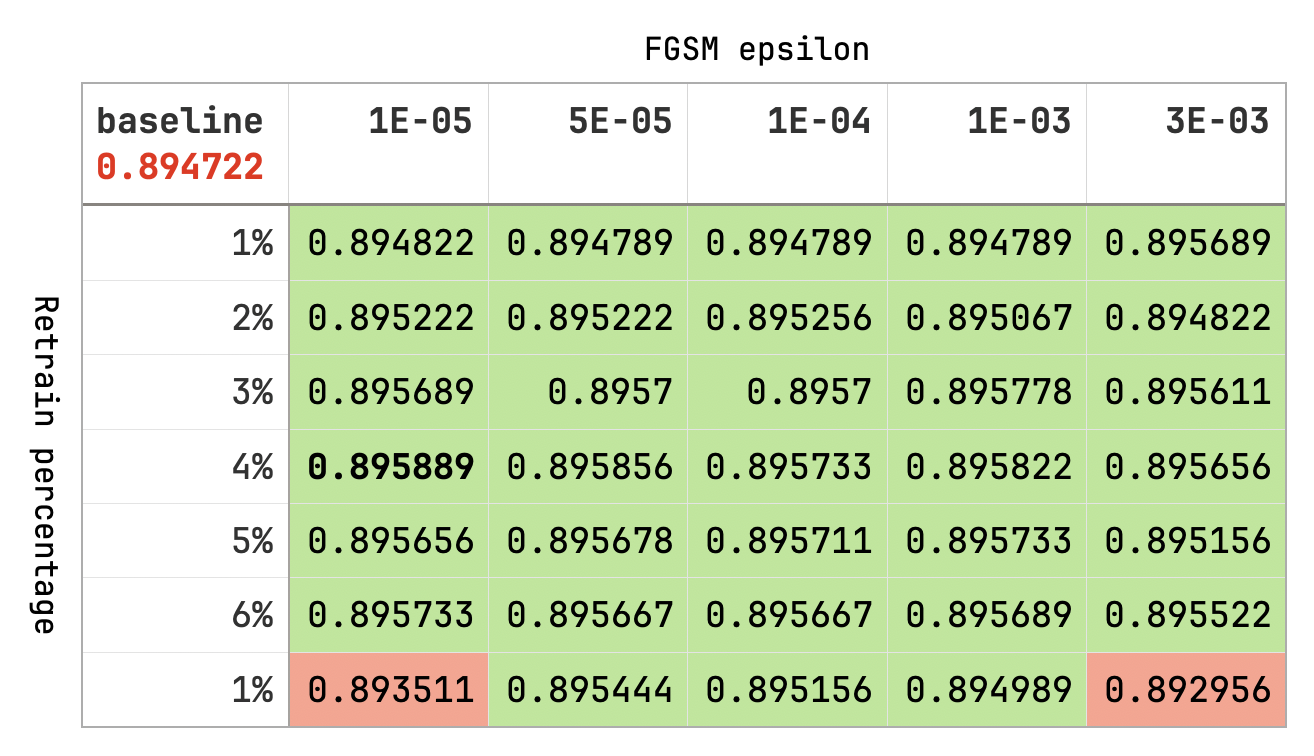
\includegraphics[width=1\textwidth]{mean-auc.png}
    % \caption{\label{fig:adv}Mean AUC of the 9 binary models}
    % \end{figure}

     \begin{table}
      \centering
      \begin{tabular}{l r r r r}
        \toprule
        \textbf{Model/\% of Data Retrain} &  1\% & 2\% & 6\% & 10\% \\
        \midrule
        Baseline(mean) & 89.30 & 89.29 & 89.30 & 89.27 \\
        Baseline(mean) + Advtrain & \textbf{89.35} & \textbf{89.41} & \textbf{89.41} & \textbf{89.41} \\
        \hline
        Baseline(Model_{S3}) & 76.50 & 76.41 & 76.53 & 76.44 \\
        Baseline(Model_{S3}) \text{+ Advtrain} & 76.50 & \textbf{76.53} & \textbf{76.64} & \textbf{76.87} \\
        \hline
        Baseline(Model_{S1}) & 94.78 & 94.82 & 94.82 & 94.95 \\
        Baseline(Model_{S1}) \text{+ Advtrain} & \textbf{95.12} & \textbf{95.45} & \textbf{95.79} & \textbf{95.71} \\
        \bottomrule
      \end{tabular}
      \caption{Retraining on Multiple Hyperparameters}
    \end{table}

    The experiment found that the best results were obtained with epsilon values of 0 to 0.003, and retrain percentages of 0.01 to 0.06 and 0.1. Overall, the experiment shows that the choice of hyper-parameters can have a significant impact on the performance of adversarial training and that careful tuning of these hyper-parameters is necessary to achieve optimal results.

  \end{block}  

\end{column}

\separatorcolumn

\begin{column}{\colwidth}

  \begin{block}{Results}

    Training the model on perturbed images forces it to make more confident and accurate predictions on perturbed images. This pushes the decision boundary away from the training data distribution and towards the true decision boundary, resulting in improved performance on test images, whether they are perturbed or not.

    \textbf{The validation AUC learning curves} indicate improvement in several models, particularly in classifying abnormalities on the sagittal plane. Additional learning curves on other evaluation metrics (accuracy, sensitivity, specifity) can be found in the Final Report. The following curves are visualized on hyperparameter:
    \begin{center}
        [$\epsilon = 1e-5, \text{retrain percentage} = 6\%$]    
    \end{center}
    
    \begin{figure}[!htp]
    \centering
    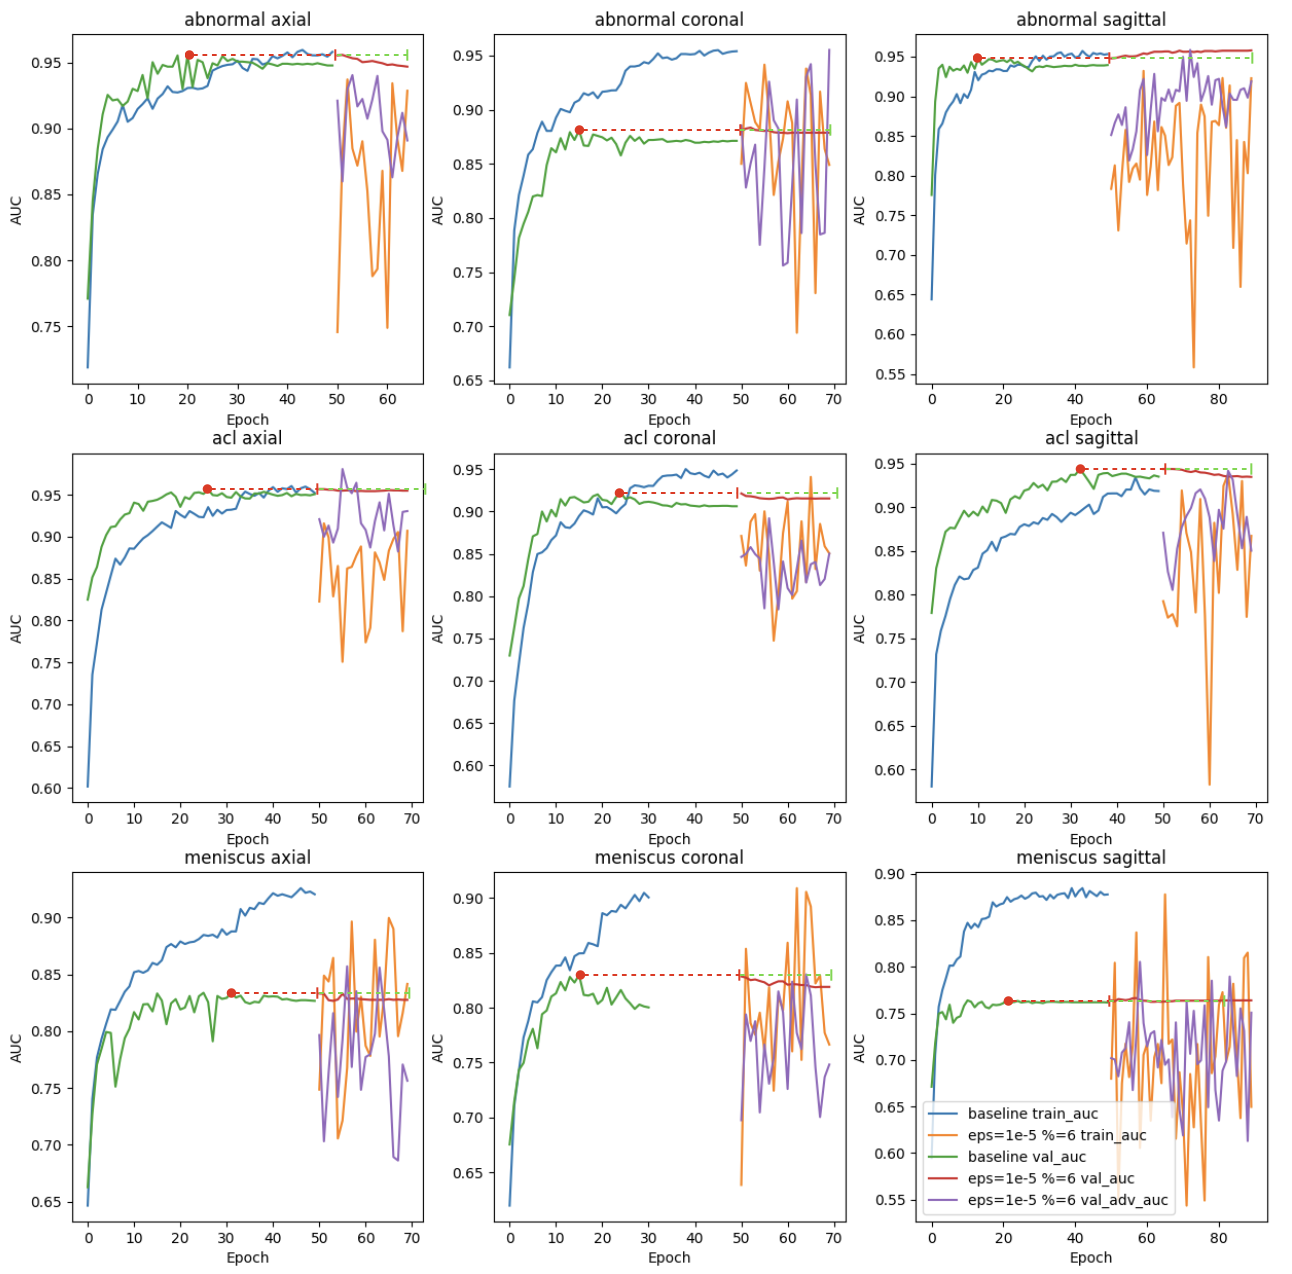
\includegraphics[width=1\textwidth]{val-auc-1.png}
    \caption{\label{fig:curve}Learning Curve on Validation AUC}
    \end{figure}

    \textbf{The ROC curves} for the nine binary models can tell how sensitive (true positive rate) and specific (false positive rate) the classifiers are for each threshold. The closer the curve is to the top-left corner of the plot, the better the classifier is.
    
    \begin{figure}[!htp]
    \centering
    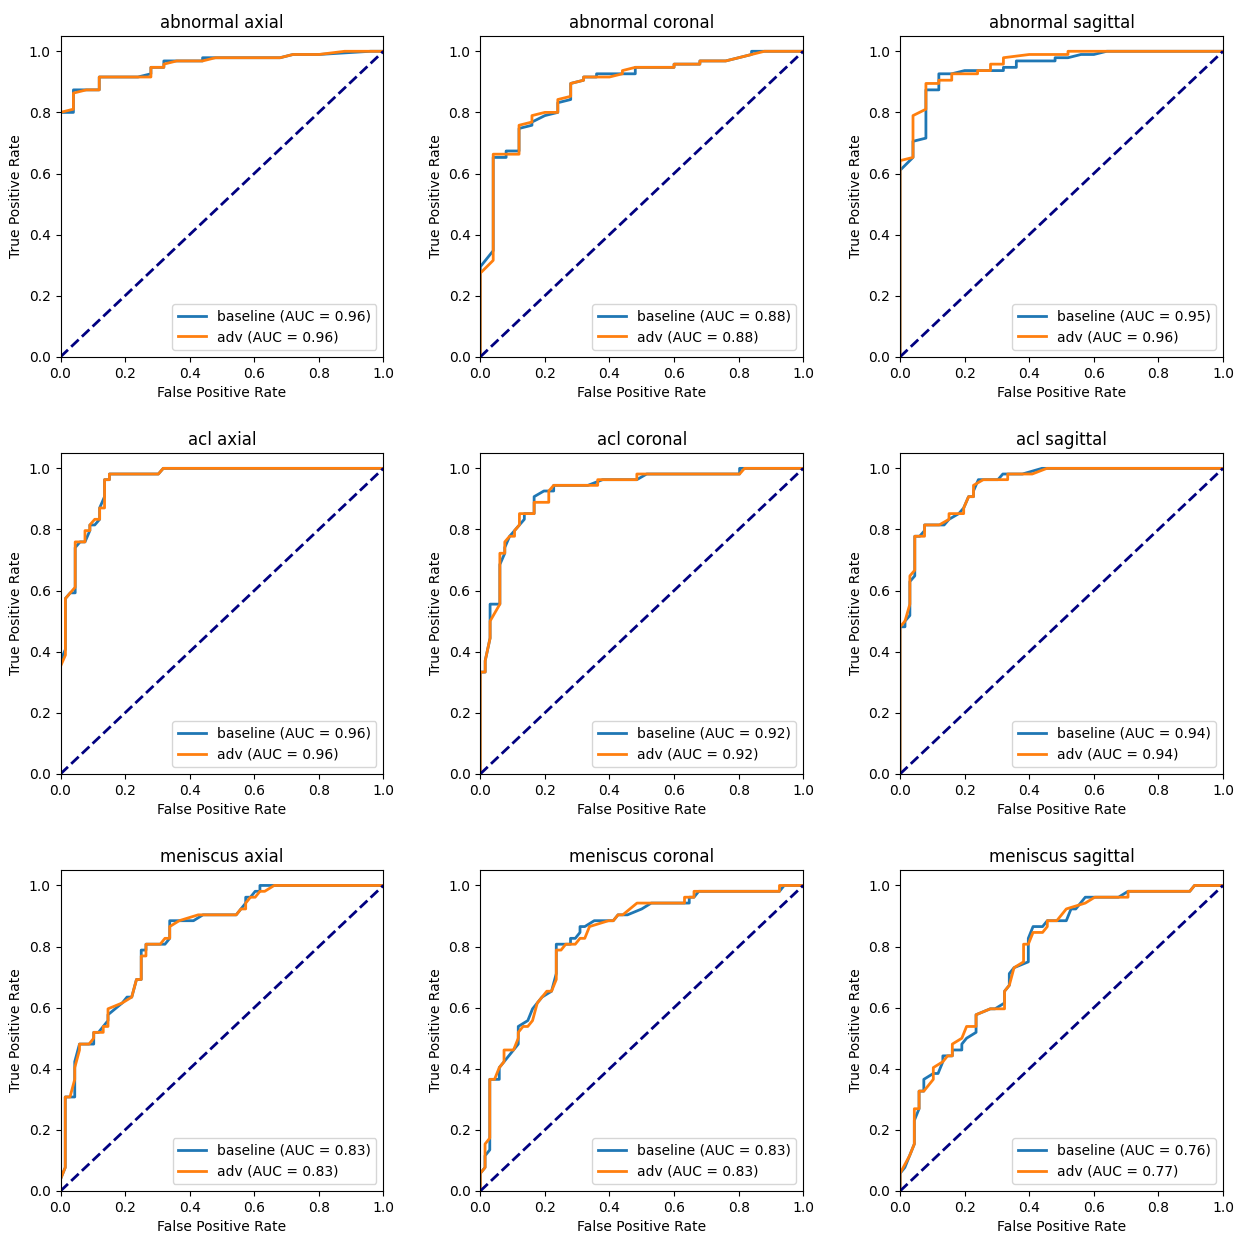
\includegraphics[width=1\textwidth]{roc_curve_MRNet_cmp-legend.png}
    \caption{\label{fig:roc}ROC Curve comparison}
    \end{figure}


  \end{block}

  \begin{block}{Conclusion}

    % According to the literature review on related works, many improvements achieved from results in classification or segmentation accuracy were presented. This work applied FGSM adversarial attack to generate adversarial examples to enlarge the original dataset. Furthermore, the work conducted adversarial training on the baseline model with a specific set of hyperparameters (retrained percentages and FGSM epsilon), besides; the work have evaluated and compared the ROC curves and multiple evaluation metrics such as AUC, accuracy, sensitivity and specificity, which related works have not conducted to the best knowledge. 

    The adversarial noise $\delta_{i}^{FGSM}$ is different from normal noise and its ability to improve the classification AUC suggests that training with adversarial examples can influence the decision boundary. This occurs by causing the model to learn from misclassified inputs that are very similar to the original data. The perturbations can shift the input to a different region of the input space, which may be closer to a different class. As a result, the decision boundary can shift, or even new decision boundaries not present before can be created.

    Adversarial training is a powerful technique for improving deep neural networks' performance on medical image analysis tasks by helping them learn more complex and informative features specific to the task. However, the finding that the ROC curve worsened for one of the classification tasks (meniscus-coronal) highlights the potential limitations and challenges of adversarial training. Careful fine-tuning of the hyperparameters and implementation details is crucial for optimizing the model's performance.

  
  \end{block}
  

\end{column}
\separatorcolumn



\end{columns}
\end{frame}


\end{document}
